% This is samplepaper.tex, a sample chapter demonstrating the
% LLNCS macro package for Springer Computer Science proceedings;
% Version 2.20 of 2017/10/04
%
\documentclass[runningheads]{llncs}
%
\usepackage{graphicx}
% Used for displaying a sample figure. If possible, figure files should
% be included in EPS format.
\usepackage{amsmath}
\usepackage{amssymb}
%
% If you use the hyperref package, please uncomment the following line
% to display URLs in blue roman font according to Springer's eBook style:
\usepackage[pagebackref=true,breaklinks=true,letterpaper=true,colorlinks,bookmarks=false]{hyperref}
\renewcommand\UrlFont{\color{blue}\rmfamily}

\begin{document}
%
\title{CALVIS: Chest, wAist and peLVIS circumference from 3D human body meshes	
as ground truth for deep learning}
%
\titlerunning{Chest, wAist and peLVIS circumference from 3D human body meshes}
% If the paper title is too long for the running head, you can set
% an abbreviated paper title here
%
\author{Yansel Gonzalez Tejeda\orcidID{0000-0003-1002-3815} \and
Helmut Mayer\orcidID{1111-2222-3333-4444}}
%
\authorrunning{Gonzalez and Mayer}
% First names are abbreviated in the running head.
% If there are more than two authors, 'et al.' is used.
%
\institute{Paris Lodron University of 
	Salzburg, Kapitelgasse 4-65020 Salzburg, Austria
\url{https://www.uni-salzburg.at}}
%
\maketitle              % typeset the header of the contribution
%
\begin{abstract}
In this paper we present CALVIS, a method to calculate chest, waist and 
pelvis circumference from 3D human body meshes. Our motivation is to use 
this data as ground truth for learning with convolutional neural networks 
(CNN). Previous work had used the large scale CAESAR dataset, determined 
$\textit{manually}$ these anthropometrical measurements or directly acquired 
them from a person. The problem is that acquiring these data is a cost and 
time consuming endeavor. In contrast our method can be used on 
3D meshes automatically. First, we slice cross sections along the Y axis of 
the mesh. Second, we calculate the cross sections length and establish a 
signature for the body represented by the mesh. Finally, using this 
signature we are able to calculate the chest, waist and pelvis 
circumference by searching for extrema. We conduct two experiments. 
In the first experiment we synthesize 10 human body meshes. Then we apply 
CALVIS to calculate chest, waist and pelvis circumference. We evaluate the 
results qualitatively. We observe that the measurements can indeed be used 
to estimate the shape of a person. The second experiment asses the 
plausibility of our approach where we use the calculated human dimensions as 
a ground truth to train a small CNN. After having trained the network with 
our data, we demonstrate that learning converges, achieving $x$ percent 
prediction error. 
Furthermore, we make the implementation of CALVIS publicly available to 
advance the field.

\keywords{Human Shape Estimation \and CNN \and Another keyword.}
\end{abstract}
%
%
%
\textbf{Motivation} 
Predicting 3D human body measurements from images is crucial in several 
scenarios 
like virtual try-on, animating, ergonomics, computational forensics and 
even health and mortality estimation. Researches had 
named this 
measurements body intuitive controls (\cite{Allen.2003}), biometric 
measurements (\cite{Sigal.2008}), body dimensions 
(\cite{DBLP:conf/bmvc/ChenRC11}, European standard EN 13402), semantical 
parameters (\cite{Yang.2014}), 
traditional anthropometric 
measurements 
(\cite{Wuhrer2011}) or only ``shape" as in human shape estimation 
(\cite{Guan.2013}, \cite{Bogo:ECCV:2016}, \cite{Loper.2015}, 
\cite{Dibra.2016a}, \cite{Pishchulin.2017}). In contrast, we assume a more 
anthropometric approach 
motivated by comprehensive compendiums like Panero and Zelnik, 1979 
\cite{panero1979human}.
Throughout this paper the term human body 
dimensions 
will be used to refer to the above measurements.

The problem of estimating human body dimensions  
having only an image is an under-constrained  (or inverse) problem. Information 
gets lost when a camera is 
used to capture the human body in 3D space to 'render' a 2D image.

To tackle this problem a supervised learning approach can be used. This approach
demands large amount of human body anthropometric measurements and is certainly 
one of the biggest challenges in the field.  Currently there 
is only one large-scale dataset, the Civilian American and 
European Surface Anthropometry Resource (CAESAR) \cite{robinette1999caesar} 
with 3D human body scans and their corresponding anthropometric measurements. 
This survey was extraordinarily large and resource intensive: around nine 
thousand people from Europe and the USA where scanned, it was conducted over 
more than five years and costed more than six million dollars.

In the past decade a noticeably amount of researchers have employed this 
dataset to investigate human shape estimation. Because the measurement 
acquiring process is resource intensive and requires large amount of human and 
material resources, this type of studies are rare and the data they offer is 
expensive. Therefore, it is important to explore alternative methods where 
human body measurements derived from real data can be obtained for 
investigation.

3D human body generative models offers such an alternative. We propose to 
synthesize 3D human body meshes using the SMPL \cite{Loper.2015} generative 
model. Once we have 
the 3D meshes we can compute chest, waist and pelvis circumference. The next 
step after obtaining the 
measurements is to use a camera model to render
images. Finally, in possession of this ground truth we can 
input this images to the learning algorithm and perform inference.

Problem statement: given a 3D human body mesh $\mathcal{M}$ we look for a 
method capable to automatically output chest, waist and pelvis circumference.

%------------------------------------------------------------------------
\section{Approach}\label{sec:approach}

In this work we synthesize 3D human meshes using the SMPL
model \cite{Loper.2015}. The generative nature of our approach establishes this 
model as starting point (and not the 3D mesh). Nevertheless, our method is 
flexible enough to begin the pipeline with a 3D mesh. In that case, an SMPL 
model can be fitted to it, using the method of (rh) for example.
This model is at its top level a skinned articulated 
model, i.e., 
consists of a 
surface mesh that mimics the skin and a skeleton related to that mesh. It is 
defined by a mean 
template shape represented by a vector of $N$ concatenated vertices 
$\mathbf{\bar{T}}$ in the zero pose, $\vec{\theta}^*$. In order 
to 
synthesize a 
new human mesh one has to deform the provided template mesh by 
setting shape parameters $\vec{\beta}$ and pose parameters $\vec{\theta}$. The 
model provides learned parameters
\begin{equation} \label{eq:smpl_params}
\Phi = \{\mathbf{\bar{T}}, \mathcal{W}, \mathcal{S}, \mathcal{J}, 
\mathcal{P}\}
\end{equation}
As mentioned above $\mathbf{\bar{T}}$ is the mean template shape. The weight 
matrix $\mathcal{W}$ represents how much the rotation of skeleton parts affects 
the vertices. In addition, the matrices $\mathcal{S}$ and $\mathcal{P}$ define 
linear functions that are used to deform $\mathbf{\bar{T}}$ and the matrix 
$\mathcal{J}$ predicts skeleton rest joint locations from vertices in the rest 
pose. We held fix these parameters during the synthesis.

\subsection{Human Body Mesh Signature}\label{subsec:hbm_signature}
Let us consider a human body mesh $\mathcal{M}$. Our method requires that 
$\mathcal{M}$ is standing with arms raised 
parallel to the 
ground at shoulder height at a $90^\circ$ angle. In the line 
of previous work \cite{Dibra.2016a}, we name this pose the zero (also 
normalized (rf)) pose $\vec{\theta}^*$. Additionally, we assume that the mesh 
has LSA orientation, e.g., x, y and z axis are positively directed from 
right-to-left, inferior-to-superior and posterior-to-anterior, respectively. If 
the mesh has another orientation we can always apply transformations to 
LSA-align it.

Intuitively, we would like to measure the chest circumference bellow the arms 
at the widest part of the torso and the waist circumference at the 
narrowest part after the chest but above the hips. This intuition is compliant 
with prior body dimensions standarised definitions (rf EN 13402 - 1). 
Similarly, the pelvis 
circumference is measured often (rf) around the widest part of hips and 
buttocks. We 
can formalize this intuition by considering the cross-sectional length of the 
2D intersection curves \cite{book.compu.topo} along the y-axis. Moreover, we 
can 
use a plane $\boldsymbol{\pi}$ parallel to the floor to intersect the mesh. 
Since $\mathcal{M}$ is 
triangulated, the boundary of this 
intersection is a collection of segments $s_i$. Therefore, we can 
determine the boundary length by specifying a point along the y-axis $j \in 
\mathbb{R}$ as
\begin{equation}
\mathcal{BL}(\mathcal{M}, \boldsymbol{\pi}, j) = \sum_{i = 
	1}^{i = n}s_i
\end{equation}

Note that for cross sections where $\boldsymbol{\pi}$ intersects the legs, two 
disconnected curves will appear. That is by no means a problem because they are 
still a collection of segment with non-zero length.

\begin{figure}[t]
	\begin{center}
		%\fbox{\rule{0pt}{2in} \rule{0.9\linewidth}{0pt}}
		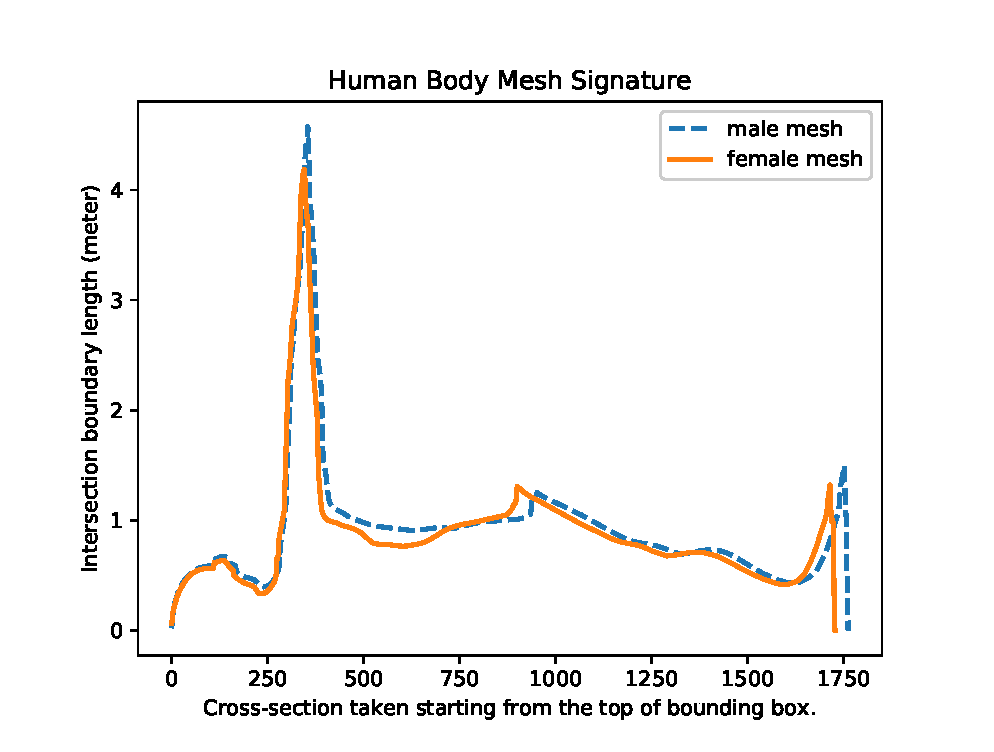
\includegraphics[width=\linewidth]{Figure_1.eps}
	\end{center}
	\caption{Human Body Mesh Signature for male and female meshes. The 
		function resembles a rotated silhouette of the human body and exhibits 
		several \textit{extrema}. See section 
		\ref{subsec:mesh_signature_extrema} for discussion of these extrema.}
	\label{fig:hbm_signature}
\end{figure}

Next, we assemble the mesh slide length vector $\vec{\mathcal{L}}$. Starting 
from the 
top $j_t$ of the bounding box we sliced iterative mesh $\mathcal{M}$ with plane 
$\boldsymbol{\pi}$ every $m$-meters until we reach the bounding box bottom 
$j_b$. For every slice at point $j$, we compute $\mathcal{BL}(j)$.

\begin{align}
\vec{\mathcal{L}}(\mathcal{M}, \boldsymbol{\pi}, m) = \mathcal{BL}(j), \, j 
\in 
\{j_t, j_t+m, \cdots, j_b\}
\end{align}

Finally, we can construct the human body \textbf{mesh signature} $\mathcal{MS}: 
\mathbb{Z}^+ \to \mathbb{R}$ that maps every slice index $k \in \{0, 1, \cdots, 
|\mathcal{L}|-1\}$ to the corresponding boundary length $\mathcal{BL}(j)$ in 
the mesh slide vector $\vec{\mathcal{L}}$.

\begin{align}\label{eq:mesh_signature}
\mathcal{MS}(k) = \mathcal{BL}(j)
\end{align}

Figure \ref{fig:hbm_signature} shows the $\mathcal{MS}$ of two meshes (male 
and female) for 
$m=0,001$ and plane $\boldsymbol{\pi}$ parallel to the floor (with normal $(0, 
1,0)$) using the library trimesh \cite{trimesh}. Note that the function as 
defined by equation \ref{eq:mesh_signature} is bounded and not continuous. It 
resembles a rotated silhouette of the human body and exhibits several 
\textit{extrema}.

\subsection{Mesh Signature Extrema}\label{subsec:mesh_signature_extrema}

By comparing neighboring values of the mesh signature $\mathcal{MS}$ as defined 
in equation \ref{eq:mesh_signature} we find several \textit{extrema}. In 
general, we expect these \textit{extrema} to be adequate features to 
calculate the human dimensions. However, there is no consensus in the 
literature regarding the method to calculate chest, waist and hip 
circumference. While Yansel et al., 2020 define waist circumference as the 

More specifically, we assume that:
\begin{enumerate}
	\item The global maximum $M_g$ represents the length of the largest path 
	around the arms. From a topographic point of view $M_g$ is the highest peak 
	of $\mathcal{MS}$. A horizontal line at height proportion $h$ of the peak 
	intersects 
	it at two points left $p_l$ and right $p_r$.
	\item The plane $\boldsymbol{\pi}$ intersects the mesh $\mathcal{M}$ at the 
	point where the left hip is located defining a path. The length of this 
	path is $P_{lh}$.	
	\item The local maximum $M_{pc}$ with largest value other than $M_g$ 
	immediately prior to $P_{lh}$ represents the pelvis circumference.	
	\item The local minimum $M_{wc}$ posterior to $p_r$ but prior to $M_{pc}$ 
	represents waist circumference.
	\item The local maximum $M_{cc}$ posterior to $p_r$ but prior to $M_{wc}$ 
	represents 
	chest circumference. If this local maximum does not exist we set $M_{cc}$ 
	to the value of the path $\mathcal{BL}(j_{cc})$ with largest value in the 
	interval $(p_l; M_{wc})$.
\end{enumerate}





%------------------------------------------------------------------------
\section{Experiments and Results}

We conduct two experiments. In the first experiment we synthesize eight (four 
female and four male) human body meshes using shape parameters provided by 
SURREAL \cite{varol17_surreal}.
The meshes reflect human figures characteristics such as bulky, slim, small and 
tall subjects. Then we apply CALVIS to calculate chest, waist and pelvis 
circumference. Since we do not have ground truth, we evaluate the results 
qualitatively by comparing our method 
with \cite{Dibra.2016b}.
The second 
experiment serves to asses the plausibility of our approach to use the 
synthetic data for deep learning. We input the calculated human 
dimensions to an artificial neural network. After having trained the network 
with our data, we show that learning converges.


%------------------------------------------------------------------------
\section{Conclusion}

The method can be optimized. Further research must be conducted.
%
% ---- Bibliography ----
%
% BibTeX users should specify bibliography style 'splncs04'.
% References will then be sorted and formatted in the correct style.
%
\bibliographystyle{splncs04}
\bibliography{egbib}
%

\end{document}
